\chapter{Atomic physics: Experimental techniques and theory}\label{chap:atomic_physics}

\lettrine[lines=3]{B}{ose--Einstein condensates} provide such a tantalising opportunity for studying quantum phenomena not only because of their interesting properties, but also because of the level of control they afford, with parameters able to be tuned and manipulated in order to investigate various regimes. Many of the same techniques which allow experimentalists such control over a \textsc{bec} are also employed in the production of \textsc{bec}.

The main experimental techniques used to create \textsc{bec} are Doppler cooling, magneto-optical, magnetic, and dipole trapping, polarisation gradient (Sisyphus) cooling, and evaporative cooling. These were discovered, perhaps by no coincidence, in roughly the same order as they are called for in a \textsc{bec} experiment, and many were first discovered along the way to the first realisations of Bose--Einstein condensation.

Section \ref{sec:cooling_and_trapping} is a whirlwind summary of these and a few other experimental techniques. Then in section \ref{sec:mean_field_theory}, I'll present some of the theory describing superfluid flow and vortices and in \textsc{bec}, which is central to the simulations of vortex tracking presented in chapter \ref{chap:velocimetry}. The final section of this chapter, section \ref{sec:the_rubidium_D_line}, will construct the detailed theory for describing the internal state of a $^{87}$Rb atom in magnetic and optical fields, considering only the first $L=0$ to $L=1$ excitation is accessible to rubidium's  sole outer-shell electron. The resulting Hamiltonian describes 32 sublevels, and forms the basis of any detailed calculations of laser cooling and trapping.

\section{Cooling, trapping, and manipulating atoms}\label{sec:cooling_and_trapping}

\subsection{Doppler cooling}\label{sec:doppler_cooling}

Doppler cooling, demonstrated in 1978 \cite{wineland_radiation-pressure_1978} is a consequence of the simple observation that atoms see the wavelength of incident light Doppler shifted depending on their velocity. For example, the electric field of a linearly polarised optical plane wave is:
\begin{align}
\vec E \propto \cos(\vec k \cdot \vec r - \omega t),
\end{align}
which for an atom moving with constant velocity $\vec v$ can be written:
\begin{align}
\vec E &\propto \cos(\vec k \cdot \vec v t - \omega t)\\
&= \cos(- \omega_\up{eff} t),
\end{align}
where $\omega_\up{eff} = \omega - \vec k \cdot \vec v$ is the effective angular frequency of the laser as seen by the atom.

This can be used to selectively transfer momentum to only fast-moving atoms, by tuning an incident laser slightly redder than would be required for a resonant absorption. If six lasers in counterpropagating pairs orthogonal to each other surround a cloud of atoms, the atoms can be cooled close to the \emph{Doppler limit} \cite[p 58]{metcalf_laser_1999}

\begin{equation}
k_\up{B} T_\up{D} = \frac{\hbar\Gamma}2
\end{equation}

where $\Gamma$ is the linewidth of the atomic transition. For the cooling transition used for Doppler cooling $^{87}$Rb\footnote{The D$_2$ line, $5\up{S}_{1/2}\rightarrow$ $5\up{P}_{3/2}$, approximately 780 nm.}, this gives $146\,\upmu$K, which is approximately a factor of a thousand too high for Bose-condensation. These atoms are also not trapped.

\subsection{Magneto-optical and magnetic trapping}

Magneto-optical trapping, first demonstrated in 1987 \cite{raab_trapping_1987} comes from the realisation that a magnetic field can be used to \emph{spatially} vary the detuning from resonance that the atoms in the above mentioned arrangement of lasers see. This is possible due to the Zeeman effect \cite{zeeman_influence_1897}, in which the wavelengths of atomic transitions are shifted in a magnetic field.

If a field profile can be found which causes the transition to come closer to resonance as the atoms move away from a central point, then it forms a trap---atoms  that stray too far from the centre will absorb more strongly and be deflected back\footnote{The polarisations of the beams are such that absorption from the inward facing beam occurs, rather than from the one that would accelerate the atom further outward!}.

The field configuration used in an anti-Helmholtz one: two coils opposite each other carrying opposing currents. The resulting magnetic field profile has a zero in the middle and increases in magnitude in all directions.

With the Doppler beams off, this magnetic field still provides a trapping potential, due to the magnetic dipole interaction:

\begin{equation}
V(\vec{r}) = -\vec \mu \cdot \vec B,
\end{equation}
where $\vec\mu$ is the atomic magnetic moment, and $\vec B$ the magnetic field. This only traps some atomic spin states, and has losses due to spin-flips \cite{brink_majorana_2006} near the field zero.

The optimal magnetic field gradient for forming a magneto-optical trap (\textsc{mot}) is lower than that required to merely hold atoms against gravity, and thus there is little if any magnetic trapping occurring in a \textsc{mot}---the trapping almost entirely results from the position-dependent rate of photon absorption caused by the Zeeman shift due to the magnetic field. To transfer atoms from a \textsc{mot} to a solely magnetic trap, the magnetic field gradient must be increased substantially.

\subsection{Optical trapping}

Optical trapping on the other hand relies on the \emph{dipole force}, in which off-resonant light shifts the energy of the eigenstates of the combined atom-light system, the so called \emph{dressed states}. This energy shift, called the \emph{light shift}, depends on the intensity of the light, and so results in a potential that spatially varies as the intensity of the light. In the limit of large detuning (compared to Rabi frequency), the resulting energy shift for an atom in a groundstate (the shift for an excited state is the same but with the opposite sign) is \cite[p 8]{metcalf_laser_1999}:

\begin{equation}
\Delta E = \frac{\hbar\Omega^2}{4\delta}
\end{equation}

where $\delta$ is the detuning from resonance and the Rabi frequency is:
\begin{equation}
\Omega=\frac{E_0}\hbar\matrixel{n^\prime}{e\hat{\vec r}}{n},
\end{equation}

where $E_0$ is the amplitude of the light's electric field and  $\matrixel{n^\prime}{e\hat{\vec r}}{n}$ is the transition dipole moment between the two states in a two-level system. This transition dipole moment can be either for two specific sublevels coupled by a laser, the calculation of which is detailed in section \ref{sec:optical_dipole_transitions}, or an overall effective transition dipole moment between two manifolds containing many sublevels, if the detuning much larger compared to the spacing between the sublevels.

With the potential proportional to $E_0^2$, and thus the light's intensity, the force the atom experiences is proportional to the light's intensity gradient. For this reason, the dipole force is also called the \emph{gradient force}. The name \emph{dipole force} comes from the fact that the force can be equivalently understood to arise from the polarisability of atoms in a light field, giving rise to a force identical to that which traps polarisable materials in optical tweezers \cite{ashkin_acceleration_1970}.

\subsection{Polarisation gradient cooling}

Polarisation gradient cooling, also called Sisyphus cooling, was proposed in 1989 \cite{dalibard_laser_1989, ungar_optical_1989} to explain experimentally measured cold atom cloud temperatures \cite{lett_optical_1989} which, at \textsc{nist} in 1988, were found to be well below the expected limit obtainable by the well understood method of Doppler cooling\footnote{As well as to explain other discrepancies between experiments and the theory of Doppler cooling, such as the optimal detuning of light being much greater than predicted.}, one of the few examples of experiments turning out better than expected. A one dimensional theory has been developed \cite{dalibard_laser_1989} which has found remarkable agreement with three dimensional experiments \cite{salomon_laser_1990}

One common configuration for Sisyphus cooling comprises two counterpropagating laser beams in each spatial dimension, both linearly polarised but with their polarisation angles perpendicular to one another. The optical field resulting from the two beams' superposition has regions of linear polarisation and of both helicities of circular polarisation, and varies between them on a length scale shorter than an optical wavelength.

The effect on multi-level atoms as they move from regions of one circular polarisation to another is that they are pumped alternately from one extreme of their spin-projection states to the other, alternately climbing and descending potential hills due to the dipole forces from the regions of different polarisations\footnote{If you consider only one polarisation of light, its intensity varies sinusoidally in space, creating a series of potential hills and wells via the dipole force}. And so, like the Greek legend of Sisyphus\footnote{Polarisation gradient cooling is but one of a family of so called `Sisyphus cooling' methods, all of which involve atoms repeatedly climbing potential hills.}, who was doomed to push a rock uphill for eternity, the atoms are climbing hills repeatedly. Due to the state dependence of the strength of the dipole forces, the atoms climb steeper hills than they descend, and are thus slowed and cooled.

This type of cooling does not work in a magnetic field; the splitting of transition frequencies makes it impossible for an atom to traverse its spin manifold on one laser frequency. For this reason the Sisyphus cooling stage is performed with magnetic fields off, though a sufficiently short period is required such that the atoms can be recaptured when the trapping field is restored.

\subsection{Evaporative cooling}\label{sec:evaporative_cooling}

The final stage of cooling is forced \textsc{rf} evaporative cooling \cite{hess_evaporative_1986, anderson_observation_1995}, which decreases the temperature of the cloud by systematically removing the hottest atoms. This is performed in a magnetic trap, which as mentioned earlier, only traps certain spin states. Evaporation proceeds by using an \emph{\rf\ knife} to induce spin flips in the atoms. The \textsc{rf} frequency is chosen such that is is only resonant with atoms some distance away from the center of the trap (via the Zeeman shift). The furthest out atoms are the most energetic, possessing the energy to climb the magnetic potential the furthest. By flipping their spins, these atoms are ejected due to the magnetic field becoming anti-trapping for them.

The cloud is given some time to rethermalise and the knife\footnote{So called because it cuts the tail off the velocity distribution of the atom cloud.} is moved inward where it removes slightly colder atoms. This is repeated until the desired compromise of lower temperature/lower atom number is reached. Usually some method is employed to prevent atoms near the center of the trap from undergoing spin flips \cite{brink_majorana_2006} as they move across the field zero. The method used in our lab is to use an optical dipole trap in combination with the magnetic trap \cite{lin_rapid_2009}, such that the coldest atoms get trapped in the dipole trap which is offset from the magnetic field zero.

\subsection{Feshbach resonances}\label{sec:feshbach}

A Feshbach resonance \cite{chin_feshbach_2010} is an enhancement of the interparticle interaction strength when when a certain magnetic field strength is applied\footnote{Feshbach resonances can also be induced optically and with \rf\, but magnetic resonances are the most commonly used.}. This phenomenon was first discovered in ultracold atoms in 1998 \cite{inouye_observation_1998}, and is now a staple of cold atom experiments.

\begin{figure}%[htb]
\begin{center}
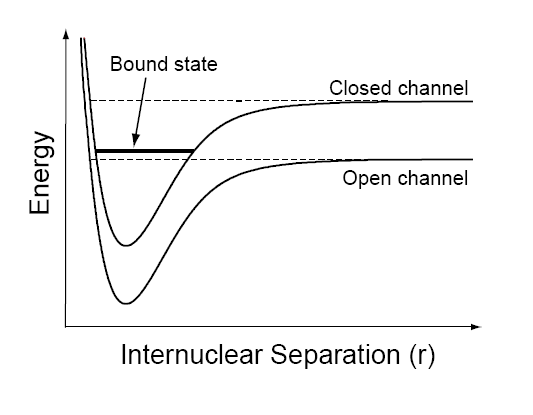
\includegraphics[width=0.5\textwidth]{figures/unsorted/feshbach.png}
\caption{When atoms approach each other with spins aligned, they are in the \emph{open channel}. In this channel they are unbound, but do not have enough energy to be free in the other channel - the \emph{closed channel}. In the close range however, the atoms may have energy corresponding to a bound (molecular) state of the closed channel, a resonance which causes a divergence in the scattering length. The energy difference between the two channels can be tuned with a magnetic field and so these resonances can be induced in a wide range of situations.}\label{fig:feshbach}
\end{center}
\end{figure}
The interparticle interaction mentioned above:

\begin{equation}
g = \frac{2\pi \hbar^2 a}{m_r}
\end{equation}
where $m_r$ is the reduced mass of a pair of the interacting particles, is dependent on a parameter $a$ called the \emph{s-wave scattering length}, which characterises low energy collisions between atoms. It is sensitive not only to what species of atoms are colliding, but also to their spin states. For each combination of spins, there is a different inter-atomic potential (called a \emph{channel}) which determines the collision dynamics (Figure \ref{fig:feshbach}).

The resulting scattering length is sensitive to any bound states of this inter-atomic potential which are near the collision energy. If the channels of different spin states are coupled via the hyperfine interaction\footnote{Requiring that the atoms in question have a nuclear magnetic moment.}, then the scattering length is also sensitive to bound states in the channels other than the one the atoms are in when they are far from each other. Due to the Zeeman effect, the energies between the different channels can be shifted with a magnetic field, and so a bound state can be shifted close to the collision energy, which causes the scattering length to diverge.

The end result is that at certain magnetic field strengths we find that atoms are much more strongly attracted to or repelled from each other.

\begin{figure}%[htb]
\begin{center}
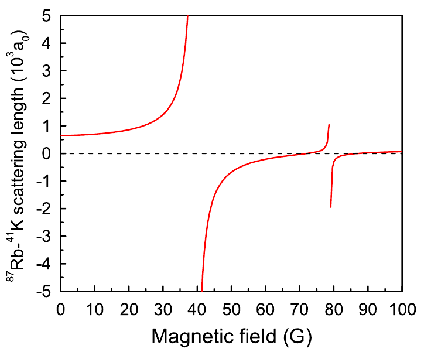
\includegraphics[width=0.5\textwidth]{figures/unsorted/feshKRb.png}
\caption{Predicted interspecies scattering length \cite{thalhammer_double_2008} as a function of magnetic field strength, for $^{41}$K and $^{87}$Rb both in their lowest energy hyperfine groundstate. The 35 gauss resonance is one of the main reasons for this pair of atoms being used in this project. It has a particularly low field strength and large width compared to most Feshbach resonances.}\label{fig:feshKRb}
\end{center}
\end{figure}

A particular Feshbach resonance of interest is shown in \figref{fig:feshKRb}, and can be used to enhance the interspecies repulsion between $^{87}$Rb and $^{41}$K. The use of this resonance is assumed for the simulations in chapter \ref{chap:velocimetry} to trap tracer particles more strongly in vortex cores of a \textsc{bec}.

\section{Mean field theory: The Gross--Pitaevskii equation and vortices}\label{sec:mean_field_theory}

Bose-condensates are described well by \emph{mean field} theory, whereby the many-body wavefunction is approximated by a product of identical single-particle wavefunctions. Indeed, that the majority of the atoms are in the same quantum state is one of the defining features of \bec. The effect of interparticle interactions is included as a nonlinear term in the Schr\"odinger equation for the single particle wavefunctions, known as the Gross--Pitaevskii equation:

\begin{equation}
\frac{\partial \Psi}{\partial t} = \left[-\frac{\hbar^2}{2m}\nabla^2 + V(\vec{x}) + g|\Psi|^2\right]\Psi,
\end{equation}

where $g$ characterises the strength of the interparticle interactions\footnote{The nonlinear constant $g$ is usually positive---having the effect of stabilising \bec s by self-repulsion.}, and $\Psi = \sqrt{N}\Psi_\up{single}$ is the single-particle wavefunction scaled by the square root of the number of particles\footnote{Thus giving it the property that $|\Psi|^2$ is the particle density.}.

In the hydrodynamic formulation of quantum mechanics \cite{madelung_quantentheorie_1927}, the flow velocity of a spatial wavefunction can be defined by considering the probability current to be a product of density and velocity. This allows us to define the superfluid velocity of a \bec\ as:
\begin{equation}
\vec v = \frac\hbar m \nabla\phi
\end{equation}
where $\phi$ is the complex phase of the condensate wavefunction $\Psi$. Integrating this velocity over any closed path $\gamma$ gives us the circulation:

\begin{align}
C &= \frac\hbar m\oint_\gamma\nabla\phi\,ds\\
  &= \frac\hbar m 2\pi n.\qquad n=0,1,2\dots
\end{align}
The fact that the circulation is quantised means that vorticity cannot exist in the condensate except in one-dimensional lines, about which the wavefunction's phase winds by a multiple of $2\pi$. These topological defects are the quantised vortices that are central to the vortex tracking simulations in chapter \ref{chap:velocimetry}.

At a vortex core, the atom density of a \bec\ must go to zero. This can be intuitively understood to arise from centrifugal forces, but is also required in order for the wavefunction to be continuous and single-valued across the core. This drop in density in the vicinity of a vortex core is exploited by the method simulated in chapter \ref{chap:velocimetry} to trap atoms within the cores.

\section{The $^{87}$Rb $\up{D}$ line}\label{sec:the_rubidium_D_line}

We atomic physicists do our theory work at an intermediate level of abstraction, at which many quantities and systems of interest can be computed and simulated with accurate models using standard quantum mechanics, but with models that are not fully a-priori. Instead, the Hamiltonians we feed to the machinery of quantum mechanics encapsulate some of the details we are not interested in or that are too hard to compute, with the link between the underlying layers of reductionism and the higher layer usually provided by experimentally measured values rather than calculations from fundamental physics. In this way we can readily compute results about the atoms we are interested in by treating them as simpler systems than they actually are, with some of the underlying details encapsulated by terms in an effective Hamiltonian for the dynamics that we are interested in.

In this section I'll summarise what the $^{87}$Rb $\up{D}$ line looks like from the perspective of a cold atom physicist, building up a Hamiltonian containing all 32 sublevels of the ground and first excited state of $^{87}$Rb including fine structure, hyperfine structure, interaction with a magnetic field, and optical transitions between states. This Hamiltonian is the starting point for any calculations regarding cooling, trapping, and coherent control of $^{87}$Rb, and for other alkali earth metals is much the same.

Much of the details of this section are drawn from references \cite{steck_rubidium_2015, steck_quantum_2017, metcalf_laser_1999, king_angular_2008, farrell_consistency_1995}, but the reader should be aware that there are considerable conventional and notational differences between different literature sources. What is presented here is summarised and framed in a way that I think is useful to an experimentalist looking to use the theory to make concrete calculations about real systems.

\subsection{Fine structure}\label{sec:fine_structure}

The rubidium 87 $\up{D}$ line refers to the first excitation available to the sole outer electron of $^{87}$Rb. Both the ground and excited state of this transition have the same principal quantum number, but different orbital angular momentum quantum numbers. Upon closer inspection, it is not just one transition between a ground state and an excited state---there are two excited states, and the two resulting transitions are called, in order of their transition frequencies, the $\up{D}_1$ and  $\up{D}_2$ lines. Thus the ground and first excited state of $^{87}$Rb are actually a ground state plus two non-degenerate excited states, once we take into account fine structure. The groundstate is an $S$ state (electronic orbital angular momentum quantum number $L=0$), called the $S_{1/2}$ state, and the two excited states are $P$ states $(L=1)$, one with the electron spin anti-aligned with its orbital angular momentum (resulting in total angular momentum quantum number $J=1/2$) and one with the electron spin aligned with its orbital angular momentum ($J=3/2$), called the $P_{1/2}$ and $P_{3/2}$ states respectively. In all of these states, $^{87}$Rb's single outer-shell electron occupies an orbital with principle quantum number $n=5$, which for brevity we leave out of the notation. The transition between $S_{1/2}$ and $P_{1/2}$ is called the $\up{D}_1$ line, with experimentally measured (angular) transition frequency $\omega_{\up{D}_1}$, and the transition between $S_{1/2}$ and $P_{3/2}$ is the $\up{D}_2$ line with angular transition frequency $\omega_{\up{D}_2}$. These transition frequencies correspond to optical wavelengths of $\lambda_{\up{D}_1} \approx 795\unit{nm}$ and $\lambda_{\up{D}_2} \approx 780\unit{nm}$\cite{steck_rubidium_2015}.

This fine structure is treated entirely empirically for our purposes, and so our base Hamiltonian for the rubidium $\up{D}$ line, taking into account only fine structure, is simply a statement of the experimentally measured energy differences between the states:

\begin{align}
\hat H_\up{fs} = 
\hbar\omega_{\up{D}_2} \hat1_{P_{3/2}} \oplus
\hbar\omega_{\up{D}_1} \hat1_{P_{1/2}} \oplus
\hat 0_{S_{1/2}},
\end{align}

where $\hat1_{P_{3/2}}$, $\hat1_{P_{1/2}}$, and $\hat 0_{S_{1/2}}$ are identity and zero operators each acting on the subspace of states within the $P_{\frac32}$, $P_{\frac12}$, and $S_{\frac12}$ manifolds respectively, and $\oplus$ is the direct sum.\footnote{Not to be confused with the Kronecker sum, with which it shares notation. The direct sum concatenates matrices as blocks, producing a larger, block-diagonal matrix with dimension equal to the \emph{sum} of the dimensions of the matrices being direct-summed, whereas the Kronecker sum is the regular sum of matrices after each has been multiplied using the Kronecker-product with identity matrices with sizes of the other matrices in the sum, producing matrices with dimension equal to the \emph{product} of those being summed.} The matrix representation $H_\up{fs}$ of $\hat H_\up{fs}$ in the basis in which it is diagonal (which we will call the $\{\ket{L_J}\}$ basis, since $L$ and $J$ are good quantum numbers\footnote{A \emph{good quantum number} is a number that can be used to label (not necessarily uniquely) an energy eigenstate, and on which the energy eigenvalue of that state depends. Saying $J$ and $L$ are good quantum numbers is saying that the eigenstates of the overall Hamiltonian are also eigenstates of $\hat L^2$ and $\hat J^2$, since eigenstates of these two operators can be specified by stating their quantum numbers $L$ and $J$.} for specifying one of the three states, which we write with the spectroscopic notation letter---$S$ or $P$---corresponding to the value of $L$ in place of its numerical value) is
\begin{align}
H_\up{fs}  = 
\left[\begin{matrix}
    \left[\begin{smallmatrix}\ddots &&\\&\hbar\omega_{\up{D}_2}&\\&&\ddots\\\end{smallmatrix} \right]\\
    & \left[\begin{smallmatrix}\ddots &&\\&\hbar\omega_{\up{D}_1}&\\&&\ddots\\\end{smallmatrix} \right]\\
    & &\left[\begin{smallmatrix}\ddots &&\\&0&\\&&\ddots\\\end{smallmatrix} \right]
\end{matrix} \right],
\end{align}
which is a block-diagonal matrix with each block also being a diagonal matrix. We have not yet specified the size of each submatrix---the size of each differs and depends on how many hyperfine and Zeeman sublevels are in that state.

This base Hamiltonian is worth singling out since the energy differences between its three states are orders of magnitude larger than any of the energy differences between hyperfine and Zeeman sublevels within them. When doing any sort of calculations or simulations then, this time-independent Hamiltonian can often be removed from the equations using an interaction picture (see Section \ref{sec:interaction_picture}), as done in Section \ref{sec:laser_cooling_simulations} in simulating laser cooling. 

\subsection{Hyperfine structure}\label{sec:hyperfine_structure}

Within each of the $S_{1/2}$, $P_{1/2}$ and $P_{3/2}$ states, the single outer-shell electron's total angular momentum $\hat {\vec J}$ has an interaction with $^{87}$Rb's nuclear angular momentum $\hat{\vec I}$. This results in multiple discrete energy levels depending on the relative orientation of the two separate angular momenta. The interaction Hamiltonian for this hyperfine structure is\footnote{Note that this expression differs from those in the cited references by a factor of $1/\hbar^2$---this is because I define the $\hat{\vec I}$ and $\hat{\vec J}$ angular momentum operators in SI units, rather than in units of $\hbar^2$.} \cite{steck_rubidium_2015, arimondo_experimental_1977}:
\begin{align}\label{eq:H_hfs}
\hat H_\up{hfs} = \frac{A_\up{hfs}}{\hbar^2} \hat{\vec I} \cdot \hat {\vec J}
+ \frac{B_\up{hfs}}{\hbar^2}\frac
{3(\hat{\vec I}\cdot\hat{\vec J})^2 + \frac32 \hat{\vec I}\cdot\hat{\vec J} - I(I + 1)J(J + 1)}
{2I(2I - 1)J(2J - 1)},
\end{align}
where $J$ is the total angular momentum quantum number of the electron, equal to either $\frac12$ or $\frac32$ depending on which state in the $\up{D}$ line we are considering, $I=\frac32$ is the total angular momentum quantum number of the nucleus, and $A_\up{hfs}$ and $B_\up{hfs}$ are empirically determined coupling constants. Here we see the boundary between the quantities we can calculate with the machinery of quantum mechanics and those that we determine empirically---this expression applies so long as $J$ and $I$ are good quantum numbers,\footnote{$J$ is a good quantum number so long as the hyperfine splitting is small compared to the spacing between the three states of the $\up{D}$ line, which it is, and $I$ is a good quantum number so long as the hyperfine splitting is small compared to the energy difference between the groundstate and the first \emph{nuclear} excited state, which it most certainly is.} and the two terms are the dipolar and quadrupolar interactions \cite{arimondo_experimental_1977} between two angular momenta, with the coupling constants determined empirically and encapsulating details that are difficult to compute a-priori, such as relativistic effects and the exact shape of the electron orbitals given the presence of inner shell electrons. For the spherically-symmetric $S_{1/2}$ groundstate, there is no quadrupolar interaction and so $B_\up{hfs}$ is only nonzero for the two $P$ excited states.\footnote{The quadrupolar term should be explicitly excluded from numerical computations of the hyperfine splitting on the $S_{1/2}$ state, as it contains a division by zero in this case, which may lead to erroneous results even if the term is subsequently multiplied by $B_\up{hfs}=0$.} The values of $A_\up{hfs}$ and $B_\up{hfs}$ for each of the three $L_J$ states of the $\up{D}$ line can be found in \cite{steck_rubidium_2015}.

For a given state of the $\up{D}$ line, we can construct the matrix representation $\oversetIJ H_\up{hfs}$ of $\hat H_\up{hfs}$ in the $\mathcal{I}\times\mathcal{J}$ basis---which we define as the basis in which both the $z$ vector components $\hat{I}_z$ and $\hat{J}_z$ of $\hat{\vec I}$ and $\hat{\vec J}$ are diagonal---by constructing matrix representations $\oversetIJ{\vec I}$ and $\oversetIJ{\vec J}$ of the operators $\hat{\vec I}$ and $\hat{\vec J}$ in that basis and then applying the expression (\ref{eq:H_hfs}). The overset ${\mathcal{I} \times \mathcal{J}}$ on each of the matrices indicates that the matrix is a representation of its respective operator in the ${\mathcal{I} \times \mathcal{J}}$ basis, so named because its basis vectors can be obtained via a Cartesian product\footnote{The different types of products available for matrices, vectors, operators, spaces, and their sets of basis vectors are rife with subfield-specific conventions and overloaded notation, leading to much ambiguity. Although `Cartesian product' connotes well what I mean here, it is still ambiguous. What I mean is that the ${\mathcal{I} \times \mathcal{J}}$ basis is the set of basis vectors $\{\left.\vec u \otimes \vec v\ \right|\ \vec u \in \mathcal{I}, \vec v\in\mathcal{J}\}$. The notation $\vec u \otimes \vec v$, which is also ambiguous, denotes the Kronecker product of two column vectors, producing a column vector with number of elements equal to the product of the number of elements in each of the two vectors---not the `outer' or `tensor' product, which would produce a matrix.} of the two sets of basis vectors from the $\mathcal{I}$ and $\mathcal{J}$ bases for the two individual nuclear and electronic angular momentum degrees of freedom, in which $\hat{I}_z$ and $\hat{J}_z$ are respectively diagonal.

To construct matrix representations of angular momentum operators in the product space basis ${\mathcal{I} \times \mathcal{J}}$, we first need their matrix representations $\oversetI{\vec I}$ and $\oversetJ{\vec J}$ in the bases of their respective subspaces, which we will write as $\vec I$ and $\vec J$ for brevity. We can then expand the two operators into the product space by applying a Kronecker product with an appropriate identity matrix to each:
\begin{align}\label{eq:kronecker_identity_I}
\oversetIJ{\vec I}
 &= \vec I \otimes \oversetJ{\mathbb{I}}\\
\label{eq:kronecker_identity_J}
\oversetIJ{\vec J}
&= \oversetI{\mathbb{I}} \otimes \vec J
\end{align}
where $\oversetI{\mathbb{I}}$ is the matrix representation of the identity operator in the $\mathcal{I}$ basis of the nuclear spin degree of freedom, equal to a $(2I+1)\times(2I+1)$ identity matrix, with $\oversetJ{\mathbb{I}}$ defined similarly for the electronic spin degree of freedom.

Each of the two matrices $\vec I$ and $\vec J$ is actually a vector of matrices, one for the angular momentum projection in each of the directions $x$, $y$ and $z$. The procedure for constructing such matrices for arbitrary total angular momentum quantum numbers is as follows.\footnote{This explicit procedure for constructing the matrix representations of these operators is useful for entering into a programming language to produce programs capable of performing atomic physics calculations for arbitrary total angular momentum quantum number $J$, without having to explicitly enter the angular momentum operators for each value of $J$, which can be tedious and prone to human error.} I'll show the procedure for constructing $J_x$, $J_y$ and $J_z$ only for an arbitrary $J$, the procedure is identical for computing the vector components of $\vec I$.

For a given total angular momentum quantum number $J$, the vector components of $\vec J$ in the $\mathcal{J}$ basis (the basis in which $J_z$ is diagonal) can be constructed using the raising and lowering operators $\hat J_+$ and $\hat J_-$. Since the action of the raising and lowering operators on an eigenstate of $J_z$ with angular momentum projection quantum number $m_J$ is to produce an adjacent ($m_J \pm 1$) eigenstate multiplied by a constant \cite[p 192]{sakurai_modern_1994}, this fact can be used to compute the nonzero matrix elements of $\hat J_+$ and $\hat J_-$ in the $\{\ket{m_J}\}$ basis (the basis kets of which we identify with the standard basis vectors\footnote{I will hereafter use the terms ``$\mathcal{J}$ basis" and ``$\{\ket{m_J}\}$ basis", and similarly for other bases, interchangeably, in the understanding that this identification of standard unit vectors with the basis kets is implied.} for a $2J+1$ dimensional space in order to define the set of concrete basis vectors $\mathcal{J}$):

\begin{align}
\matrixel{m_J + 1}{\hat J_+}{m_J} &= \hbar\sqrt{J(J + 1) - m_J(m_J + 1)}, \qquad -J \leq m_J < J,\\
\matrixel{m_J - 1}{\hat J_-}{m_J} &= \hbar\sqrt{J(J + 1) - m_J(m_J - 1)}, \qquad -J < m_J \leq J,
\end{align}
and therefore compute explicit matrices for $J_+$ and $J_-$ in the $\{\ket{m_J}\}$ basis:\footnote{We're using the standard convention of ordering the eigenkets $\{\ket{m_J}\}$ in descending order of $m_J$. This is at odds with the computer programming convention of looping over most indices in ascending order, and so care should be taken when constructing these matrices in a computer program.}
\begin{align}
J_+ &=
\left[\begin{smallmatrix}
0 &  \matrixel{J}{\hat J_+}{J - 1} & 0 & \hdots\\
\hdots & 0 & \matrixel{J - 1}{\hat J_+}{J - 2} & 0 & \hdots\\
& & \ddots & \ddots & \ddots\\
 & & \hdots & 0 & \matrixel{ -J + 2}{\hat J_+}{-J + 1} & 0\\
 & & & \hdots & 0 & \matrixel{ -J + 1}{\hat J_+}{-J}\\
 & & & & \hdots & 0\\
\end{smallmatrix} \right],\\
J_- &=
\left[\begin{smallmatrix}
    0 & \hdots \\
    \matrixel{J - 1}{\hat J_-}{J} & 0 & \hdots\\
    0 & \matrixel{J - 2}{\hat J_-}{J - 1} & 0 & \hdots\\
    \hdots & 0 & \matrixel{J - 3}{\hat J_-}{J - 2} & 0 & \hdots\\
    & & \ddots & \ddots & \ddots\\
    & & \hdots & 0 & \matrixel{-J}{\hat J_-}{-J + 1} & 0 \\
\end{smallmatrix} \right],
\end{align}
both of which have nonzero values along only one non-main diagonal adjacent to the main diagonal, and which form a Hermitian conjugate pair (or indeed, a transpose pair, since all elements are real). The matrix representations of $\hat J_x$ and $\hat J_y$ can then be computed by rearranging the defining expressions for $\hat J_+$ and $J_-$;
\begin{align}
\hat J_+ = \hat J_x + \ii \hat J_y,\\
\hat J_- = \hat J_x - \ii \hat J_y,
\end{align}
for $\hat J_x$ and $\hat J_y$, and then applying the result to our matrix representations of $\hat J_+$ and $\hat J_-$ to obtain matrix representations $J_x$ and $J_y$ of $\hat J_x$ and $\hat J_y$ in the $\{\ket{m_J}\}$ basis:
\begin{align}
J_x &= \frac{J_+ + J_-}{2},\\
J_y &= \frac{J_+ - J_-}{2\ii}.
\end{align}
Finally, since $\{\ket{m_J}\}$ is the eigenbasis of $J_z$ with eigenvalues $\{\hbar m_J\}$, the matrix representation of $J_z$ in the $\mathcal{J}$ basis is simply the diagonal matrix of eigenvalues:
\begin{align}
J_z = \left[\begin{smallmatrix}
\hbar J\\
& \hbar (J - 1)\\
& & \ddots\\
& & & \hbar (- J + 1)\\
& & & & -\hbar J\\
\end{smallmatrix} \right].
\end{align} 
We can also construct the matrix representation $J^2$ of the total (squared) angular momentum operator $\hat J^2$ as
\begin{align}
J^2 = J_x^2 + J_y^2 + J_z^2, 
\end{align} 
or equivalently
\begin{align}
J^2 = J(J+1)\hbar^2 \oversetJ{\mathbb{I}},
\end{align}
since every $m_J$ state is an eigenstate of the $J^2$ operator with eigenvalue $J(J+1)\hbar^2$.

The above prescription can be used to produce matrix representations of angular momentum operators $J_x$, $J_y$, $J_z$ and $J^2$ for any integer or half-integer total angular momentum quantum number $J$. The three components can be considered a vector of matrices, $\vec J$, for the vector angular momentum operator $\hat {\vec J}$. Below is a Python function that computes these matrices as well as the corresponding eigenvectors:

\python{code_listings/angular_momentum_operators.py}

Using the above prescription to construct a matrix representation of the $\hat J$ operator with $J=\frac12$ for the $S_{1/2}$ and $P_{1/2}$ states, or $J=\frac32$ for the $P_{3/2}$ state, and to construct a matrix representation of the $\hat I$ operator with $I=\frac32$, we can explicitly construct a matrix representation of the hyperfine interaction Hamiltonian for any state of the $^{87}$Rb $\up{D}$ line. Remaining is to obtain the matrix representations of the two operators in the $\mathcal{I}\times\mathcal{J}$ product space basis using \eqref{eq:kronecker_identity_I} and \eqref{eq:kronecker_identity_J}, and then we can apply \eqref{eq:H_hfs} to our matrices to obtain the matrix representation $\oversetIJ H_\up{hfs}$ of $\hat H_\up{hfs}$ for a given $J$ corresponding to one of the three states on the $\up{D}$ line:
\begin{align}\label{eq:H_hfs_matrix}
\oversetIJ H_\up{hfs} = \frac{A_\up{hfs}}{\hbar^2}
\oversetIJ{\vec I} \cdot
\oversetIJ{\vec J}
+ \frac{B_\up{hfs}}{\hbar^2}\frac
{3(\oversetIJ{\vec I}\cdot
\oversetIJ{\vec J})^2
+ \frac32 \oversetIJ{\vec I}\cdot
\oversetIJ{\vec J}
 - I(I + 1)J(J + 1)}
{2I(2I - 1)J(2J - 1)},
\end{align}
where the products of vector components within the dot products are computed with ordinary matrix multiplication. Alternatively, one can use the matrices in their individual subspaces rather than their equivalents in the product space, so long as one interprets the dot products as ``Kronecker dot products":
\begin{align}\label{eq:H_hfs_matrix_kron}
\oversetIJ H_\up{hfs} = \frac{A_\up{hfs}}{\hbar^2}
\vec I \krondot \vec J
+ \frac{B_\up{hfs}}{\hbar^2}\frac
{3(\vec I \krondot \vec J)^2
+ \frac32 \vec I \krondot \vec J
 - I(I + 1)J(J + 1)}
{2I(2I - 1)J(2J - 1)},
\end{align}
where $\krondot$ is the Kronecker dot product:
\begin{align}
\vec I \krondot \vec J \equiv I_x \otimes J_x + I_y \otimes J_y + I_z \otimes J_z.
\end{align}

In the above way one can construct an explicit matrix representation of $\hat H_\up{hfs}$ in the $\mathcal{I} \times \mathcal{J}$ basis for the hyperfine interaction for a given $L_J$ state of the $\up{D}$ line.

\subsubsection{Column vectors in the $\mathcal{I}\times\mathcal{J}$ basis}

Because the matrix representations $\vec I$ and $\vec J$ of the electron and nuclear angular momentum operators were constructed in the $\{\ket{m_I}\}$ and $\{\ket{m_I}\}$ bases of their respective subspaces, the matrices we have constructed are in the basis $\mathcal{I}\times\mathcal{J}$ with basis vectors:
\begin{align}
\mathcal{I}\times\mathcal{J} = \left\{\left. \ket{m_I\ m_J} \ \right| \ \ket{m_I} \in \{\ket{m_I}\}, \ket{m_J} \in \{\ket{m_J}\}\right\},
\end{align}
where $\ket{m_I\ m_J} = \ket{m_I} \otimes \ket{m_J}$. The vector representation $\vec\psi$ of a state vector $\ket{\psi}$ in this basis is:
\begin{align}
\vec \psi = \left[\begin{smallmatrix}
\braket{m_I=I\ m_J=J}{\psi}\\
\braket{m_I=I\ m_J=J-1}{\psi}\\
\vdots\\
\braket{m_I=I\ m_J=-J}{\psi}\\
\braket{m_I=I-1\ m_J=J}{\psi}\\
\braket{m_I=I-1\ m_J=J-1}{\psi}\\
\vdots\\
\vdots\\
\braket{m_I=-I\ m_J=-J}{\psi}\\
\end{smallmatrix}\right].
\end{align}
The hyperfine Hamiltonian is not diagonal in the $\{\ket{m_I\ m_J}\}$ basis. The basis in which it is diagonal---the $\{\ket{F\ m_F}\}$ basis---will be discussed in section \ref{sec:the_F_mF_basis}.

\subsection{Zeeman sublevels}\label{sec:zeeman_sublevels}

The states differing only in their $m_F$ quantum numbers---called Zeeman sublevels---are degenerate in energy with respect to the hyperfine Hamiltonian, but an external magnetic field lifts this degeneracy. The Zeeman effect \cite{zeeman_influence_1897, steck_rubidium_2015} results in an energy shift proportional to the external magnetic field $\vec B$ and to a system's magnetic moment $\vec \mu$:
\begin{align}
V = - \vec\mu\cdot\vec B.
\end{align}
Our atom is a composite particle, made of a nucleus with its own intrinsic magnetic moment, an electron with its own intrinsic one as well, and a contribution from the orbital motion of the electron about the nucleus. Each magnetic moment is proportional to the angular momentum of the subsystem in question, with the proportionality constants, called Land\'e g-factors written as dimensionless multiples of $-\mu_B/\hbar$, where $\mu_B$ is the Bohr magneton.\footnote{We are using the sign convention that defines the Lande $g$-factor $g_J$ for the electron as positive.} Since $J$ is a good quantum number so long as energy shifts are smaller than the (large) energy spacing between the three $L_J$ states of the $\up{D}$ line, on the level we work we don't consider the electron spin and orbital angular momenta separately, rather we encapsulate them with a single, empirically determined Land\'e g-factor $g_J$ \cite{steck_rubidium_2015} for the magnetic moment of the electron in each of the three $L_J$ states. Similarly we consider the nucleus as a single spin with an experimentally determined $g_I$ \cite{steck_rubidium_2015}, resulting in a Zeeman Hamiltonian:
\begin{align}
\hat H_\up{Z} & = -\hat{\vec \mu} \cdot \vec B\\
&= -\left(\hat{\vec \mu}_I + \hat{\vec \mu}_J\right) \cdot \vec B\\
&=\left(\frac{g_I\mu_B}{\hbar} \hat{\vec I} + \frac{g_J\mu_B}{\hbar} \hat{\vec J}\right) \cdot \vec B.\label{eq:H_Z}
\end{align}
Separate $g_S$ and $g_L$ values are known and can be used in two terms instead of the one containing $\hat{\vec J}$ above if $J$ is not a good quantum number, but in the regime we work that is not usually the case (and if it were, the fine and hyperfine structure Hamiltonians above would also be inadequate since they assume that $J$ is a good quantum number). If $J$ is a good quantum number then it is more accurate to use the above expression with empirically measured $g_J$ values, since they encapsulate QED effects and corrections due to the multi-electron structure of $^{87}$Rb that are not captured by the simple Zeeman Hamiltonian with separate $\hat{\vec S}$ and $\hat{\vec L}$ terms \cite{steck_rubidium_2015}. 

If the energy shifts from the Zeeman effect are small compared to the hyperfine spitting, then $F$ (the total spin quantum number, defined in the next section) is a good quantum number and a given hyperfine level can be treated as a single magnetic moment subject to the Zeeman Hamiltonian:
\begin{align}
\hat H_\up{Z\,lin} = \frac{g_F\mu_B}{\hbar} \hat{\vec F} \cdot \vec B,
\end{align}
where \cite{steck_rubidium_2015}
\begin{align}
g_F = g_J\frac{F(F+1) - I(I+1) + J(J+1)}{2F(F+1)}
    + g_I\frac{F(F+1) + I(I+1) - J(J+1)}{2F(F+1)}.
\end{align}
The direction in which each Zeeman sublevel shifts in energy for small magnetic fields is depicted in \figref{fig:D_line}. Experimentally, Zeeman shifts that depart from this linear regime are not infrequently encountered, and so it is an approximation that cannot always be made.

An explicit matrix representation $\oversetIJ{H}_\up{Z}$ of $\hat H_\up{Z}$ in the $\{\ket{m_I\ m_J}\}$ basis for each of the three $L_J$ states of the $\up{D}$ line can be constructed by applying \eqref{eq:H_Z} to the matrix representations of $\hat{\vec I}$ and $\hat{\vec J}$ in that basis: 
\begin{align}\label{eq:Zeeman_hamiltonian}
\oversetIJ{H}_\up{Z} &= -\oversetIJ{\vec\mu}\cdot \vec B,
\end{align}
where
\begin{align}\label{eq:magnetic_moment_operator}
\oversetIJ{\vec\mu} &=
-\frac{g_I\mu_B}{\hbar} \oversetIJ{\vec I}
- \frac{g_J\mu_B}{\hbar} \oversetIJ{\vec J}\\
&= -\frac{g_I\mu_B}{\hbar} \vec I \otimes \oversetJ{\mathbb{I}}
- \frac{g_J\mu_B}{\hbar} \oversetI{\mathbb{I}} \otimes \vec J.
\end{align}

\subsection{Putting it all together: the $\{\ket{F\ m_F}\}$ basis}\label{sec:the_F_mF_basis}

So far we have described how to construct a matrix representation of the fine structure Hamiltonian for the three $L_J$ states of the $^{87}$Rb $\up{D}$ line, as well as matrix representations of each state's hyperfine and Zeeman Hamiltonians, these latter two in the same $\{\ket{m_I\ m_J}\}$ basis. In the subspaces of each of the three $L_J$ states then, we can sum together the hyperfine and Zeeman Hamiltonians to form (a matrix representation of) a Hamiltonian that takes interactions into account:
\begin{align}
\oversetIJ H_{P_{3/2}} &=
  \oversetIJ H_{\up{hfs}\,P_{3/2}} + \oversetIJ H_{\up{Z}\,P_{3/2}},\\
\oversetIJ H_{P_{1/2}} &=
  \oversetIJ H_{\up{hfs}\,P_{1/2}} + \oversetIJ H_{\up{Z}\,P_{1/2}},\\
\oversetIJ H_{S_{1/2}} &=
  \oversetIJ H_{\up{hfs}\,S_{1/2}} + \oversetIJ H_{\up{Z}\,S_{1/2}},
\end{align}
where the subscripts $P_{3/2}$, $P_{1/2}$, and $S_{1/2}$ on the terms on the right hand side indicate that the expressions for the matrix elements of the hyperfine and Zeeman Hamiltonians are to be evaluated using the specific values of $J$, $A_\up{hfs}$, $B_\up{hfs}$, and $g_J$ relevant to that state. The total Hamiltonian for the $\up{D}$ line including fine structure, hyperfine structure and the Zeeman interaction is then
\begin{align}
\hat H &= \hat H_\up{fs} +
    \left(\hat H_{P_{3/2}} \oplus \hat H_{P_{1/2}} \oplus \hat H_{S_{1/2}} \right)\\
\Rightarrow \hat H &= 
\left(\hbar\omega_{D_2}\hat 1_{P_{3/2}} + \hat H_{P_{3/2}}\right) \oplus
\left(\hbar\omega_{D_1}\hat 1_{P_{1/2}} + \hat H_{P_{1/2}}\right) \oplus \hat H_{S_{1/2}},
\end{align}
the matrix representation of which in the $\{\ket{L\ J\ m_I\ m_J}\}$ basis is the block diagonal matrix
\begin{align}
\oversetIJ H_{\up{D}\,^{87}\up{Rb}}  = 
\left[\begin{matrix}
    \left[\begin{smallmatrix}
        \hbar\omega_{\up{D}_2} + \oversetIJ  H_{P_{3/2}}\\
    \end{smallmatrix} \right]\\
    & \left[\begin{smallmatrix}
        \hbar\omega_{\up{D}_1} + \oversetIJ  H_{P_{1/2}}\\
      \end{smallmatrix} \right]\\
    & &\left[\begin{smallmatrix}
        \oversetIJ  H_{S_{1/2}}\\
        \end{smallmatrix} \right]\\
\end{matrix} \right],
\end{align}
where addition of scalars with matrices implies the addition of a scalar multiple of the appropriately sized identity matrix.

While $\oversetIJ H_{\up{D}\,^{87}\up{Rb}}$ is a block diagonal matrix, each of the three submatrices is not diagonal, since $m_I$ and $m_J$ are not good quantum numbers for the hyperfine interaction (though they are good quantum numbers for the Zeeman interaction and hence $\oversetIJ  H_{\up{D}\,^{87}\up{Rb}}$ becomes approximately diagonal at high magnetic field). Once one has constructed $\oversetIJ  H_{\up{D}\,^{87}\up{Rb}}$ or its submatrices, there are two other bases one might consider transforming the submatrices into depending on the circumstances. One is the $\Sigma\mathcal{F} = \{\ket{F\ m_F}\}$ basis\footnote{The name $\Sigma\mathcal{F}$ refers to the fact that this is the basis that lends itself to the interpretation of the total space being the direct sum of subspaces, each of which has a well defined $F$ quantum number. So if $\mathcal{I}\times\mathcal{J}$ is a basis for a product space with $(2I+1)\times(2J+1)$ dimensions, then $\Sigma \mathcal{F}$ is a basis for a \emph{sum space} with $\sum_i (2F_i + 1)$ dimensions, where $F_i$ ranges from $\abs{I-J}$ to $I+J$ in integer steps. The product and sum bases have the same dimensionality and span the same space, so the difference is only in the identification and composition of their component subspaces.}, in which the matrix representation of the hyperfine interaction is diagonal. The matrix representation of the Zeeman Hamiltonian is also approximately diagonal in the $\{\ket{F\ m_F}\}$ basis, so long as one is in the linear Zeeman regime. Furthermore, the transition dipole moments for optical transitions are most easily calculated in the $\{\ket{L_J\ F\ m_F}\}$ basis, as we'll see in the next subsection. For these reasons the $\{\ket{F\ m_F}\}$ basis is the most commonly used and referred to.

The $\{\ket{F\ m_F}\}$ basis is defined as the simultaneous eigenbasis of the $\hat F^2$ and $\hat F_z$ operators, which are the total (squared) and $z$ component of the total angular momentum operator $\hat{\vec{F}} = \hat{\vec{I}} + \hat{\vec{J}}$, the matrix forms $F^2$ and $F_z$ of which in the $\ket{m_I\ m_J}$ basis can be constructed from the matrix forms of the individual angular momentum operators:
\begin{align}
\oversetIJ{\vec F} &= \oversetIJ{\vec I} + \oversetIJ{\vec J}\nonumber\\
& = \vec I \otimes \oversetJ{\mathbb{I}} + \oversetI{\mathbb{I}} \otimes \vec J\\
\oversetIJ{F_z} &= \oversetIJ {I_z} + \oversetIJ {J_z}\nonumber\\
& = I_z \otimes \oversetJ{\mathbb{I}} + \oversetI{\mathbb{I}} \otimes J_z\\
\oversetIJ {F^2} &= \oversetIJ{\vec F}\cdot\oversetIJ{\vec F}
\end{align}

The $\{\ket{F m_F}\}$ basis allows the eigenstates of the hyperfine interaction to be labelled with $F$ and $m_F$ quantum numbers. For a state of the $^{87}$Rb $\up{D}$ line with electron total angular momentum quantum number $J$, there are $1+J+I - \abs{(I - J)}$ hyperfine levels, with $F$ quantum numbers running from $\abs{I - J}$ to $I + J$. Within each hyperfine level there are $2F + 1$ degenerate states with different $m_F$ quantum numbers ranging from $-F$ to $F$. This results in a total of 32 possible states for the rubidium $\up{D}$ line, a schematic of which is shown in \figref{fig:D_line}.

\begin{figure}%[htb]
\begin{center}
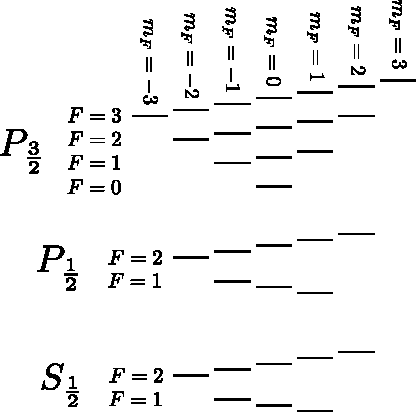
\includegraphics[width=0.5\textwidth]{figures/atomic_physics/D_line.pdf}
\caption{The 32 states of the rubidium 87 $\up{D}$ line, ordered vertically by energy (not to scale) in a small magnetic field. At zero magnetic field, Zeeman sublevels sharing a common $F$ quantum number and within the same hyperfine level are degenerate. At small magnetic fields this degeneracy is lifted, with state energies shifting in the directions depicted. However, $F$ is no longer a good quantum number at nonzero magnetic field, as most of the non-degenerate sublevels are actually equal to linear combinations of two states of different $F$ quantum numbers. Nevertheless at low magnetic fields the states are labelled using $F$ anyway, since one $F$ state dominates the linear combination, and at higher magnetic fields the states are labelled using an index $\alpha$, equal to the value of $F$ of the state that would dominate the superposition if the field were smoothly reduced to zero. $m_F$ remains a good quantum number at nonzero magnetic field however, and so at all fields a state can be specified by the numbers $L$, $J$, $\alpha$ (equal to $F$ at small field) and $m_F$.} \label{fig:D_line}
\end{center}
\end{figure}

To transform each submatrix between the $\{\ket{m_I\ m_J}\}$ and $\{\ket{F\ m_F}\}$ bases, we use a unitary matrix whose elements are Clebsch--Gordan coefficients, each defined as the inner product of a $\ket{F\ m_F}$ state with a $\ket{m_I\ m_J}$ state (written in full as $\ket{I\ m_I\ J\ m_J}$), and calculable as \cite{steck_rubidium_2015}
\begin{align}\label{eq:ClebschGordanCoeffs}
\braket{I\ m_I\ J\ m_J}{F\ m_F} &=
(-1)^{I - J + m_F}\sqrt{2F + 1}
\left(\begin{matrix}
I & J & F\\
m_I & m_J & -m_F\\
\end{matrix}\right)
\end{align}
where the object in parentheses is a Wigner $3$-j symbol. The Clebsch--Gordan coefficients are real: $\braket{F\ m_F}{I\ m_I\ J\ m_J} = \braket{I\ m_I\ J\ m_J}{F\ m_F}$, and are zero unless $m_I + m_J = m_F$.
Given that the possible range of the $F$ quantum number is from $\abs{I - J}$ to $I + J$, and the possible range of $m_F$ quantum numbers is from $-F$ to $F$ for each $F$ (both in integer steps), an explicit construction of the unitary matrix $U_\up{CG}$ of Clebsch--Gordan coefficients, in the convention where the column vectors in the $\{\ket{F\ m_F}\}$ basis have $F$ running from its highest value to lowest from top to bottom, and $m_F$ also running from highest to lowest within each value of $F$, (omitting $I$ and $J$ for brevity) is:
\begin{align}
U_\up{CG} = \left[\begin{smallmatrix}
\braket{m_I=I\ m_J=J}{F=I+J\ mF=F} & \hdots &
\braket{m_I=I\ m_J=J}{F=I+J\ m_F=-F} & \hdots &\hdots &
\braket{m_I=I\ m_J=J}{F=\abs{I - J}\ m_F=-F}\\
\vdots\\
\braket{m_I=-I\ m_J=J}{F=I+J\ mF=F} & & \ddots & & & \vdots\\
\vdots\\
\vdots\\
\braket{m_I=-I\ m_J=-J}{F=I+J\ mF=F} & & \hdots & & &
\braket{m_I=-I\ m_J=-J}{F=\abs{I - J}\ m_F=-F}\\
\end{smallmatrix}\right].
\end{align}
This the matrix that takes vectors from the $\{\ket{F\ m_F}\}$ basis to the $\{\ket{m_I\ m_J}\}$ basis, so its Hermitian conjugate $U^\dagger_\up{CG}$ is needed for the inverse transformation (which is equal to the transpose since the matrix elements are real). Within the convention we're using to order the matrix elements, the vector representation $\vec\psi$ of a state vector $\ket{\psi}$ in the $\{\ket{F\ m_F}\}$ basis of one of the $L_J$ states is:
\begin{align}
\vec \psi = \left[\begin{smallmatrix}
\braket{F=I+J\ m_F=F}{\psi}\\
\braket{F=I+J\ m_F=F-1}{\psi}\\
\vdots\\
\braket{F=I+J\ m_F=-F}{\psi}\\
\braket{F=I+J-1\ m_F=F}{\psi}\\
\braket{F=I+J-1\ m_F=F-1}{\psi}\\
\vdots\\
\vdots\\
\braket{m_F=\abs{I-J}\ m_F=-F}{\psi}\\
\end{smallmatrix}\right].
\end{align}

Each submatrix of the total Hamiltonian for the $\up{D}$ line can be transformed into its $\{\ket{F\ m_F}\}$ basis by using a unitary matrix of Clebsch--Gordan coefficients with the appropriate value of $J$, yielding a total Hamiltonian for the rubidium 87 $\up{D}$ line in the $\{\ket{L_J\ F\ m_F}\}$ basis:
\begin{align}
\oversetF{H}_{\up{D}\,^{87}\up{Rb}}
&= \left[\begin{matrix}
    \left[\begin{smallmatrix}
        \hbar\omega_{\up{D}_2}+U^\dagger_{\up{CG}\,3/2}
        \oversetIJ H_{P_{3/2}}U_{\up{CG}\,3/2}\\
        \end{smallmatrix} \right]\\
    & \left[\begin{smallmatrix}
        \hbar\omega_{\up{D}_1}+U^\dagger_{\up{CG}\,1/2}
        \oversetIJ H_{P_{1/2}}U_{\up{CG}\,1/2}\\
      \end{smallmatrix} \right]\\
    & &\left[\begin{smallmatrix}
        U^\dagger_{\up{CG}\,1/2} 
        \oversetIJ H_{S_{1/2}} U_{\up{CG}\,1/2}\\
    \end{smallmatrix} \right]\\
\end{matrix} \right]\\
&= \left[\begin{matrix}
    \left[\begin{smallmatrix}
        \hbar\omega_{\up{D}_2} +
        \oversetF H_{P_{3/2}}\\
        \end{smallmatrix} \right]\\
    & \left[\begin{smallmatrix}
        \hbar\omega_{\up{D}_1} +
        \oversetF H_{P_{1/2}}\\
      \end{smallmatrix} \right]\\
    & &\left[\begin{smallmatrix}
        \oversetF H_{S_{1/2}}\\
    \end{smallmatrix} \right]\\
\end{matrix} \right]
\end{align}
where the additional subscripts on the unitary matrices indicates the value of $J$ used in its construction. Armed with the $\{\ket{F, m_F}\}$ basis, we have little remaining reason to use the $\{\ket{m_I\ m_J}\}$ basis any more.

Here is a recap of what we have taken into account with our model of the Rubidium $\up{D}$ line:
\begin{itemize}
    \item The two lowest quantum numbers $L=0$ and $L=1$ of the electron's orbital angular momentum. This yields the $S$ groundstate and $P$ excited state.
    \item Fine structure: the two possible orientations of the electron's spin with respect to its orbital angular momentum. This splits the $P$ excited state into two states, $P_{1/2}$ and $P_{3/2}$, and leaves the $S$ groundstate as the single state $S_{1/2}$. The energies of these three states are determined entirely empirically---without any modelling of the fine structure.
    \item Hyperfine structure: The possible orientations of the electron's total angular momentum with respect to the nuclear angular momentum. This splits each state so far into $1+J+I - \abs{(I - J)}$ hyperfine states. The hyperfine interaction is treated semi-empirically, using an analytic form of the hyperfine interaction but with empirically determined coupling constants within each of the three $L_J$ states of the $\up{D}$ line. 
    \item Zeeman effect: the possible orientation of the angular momenta $\hat{\vec I}$ and $\hat{\vec J}$---or at low field their sum $\hat{\vec F}$---onto an external magnetic field. The Zeeman Hamiltonian is modelled analytically, but with empirically determined Land\'e $g$ factors for each of the three $L_J$ states of the $\up{D}$ line. 
\end{itemize}

The above considerations allow us to construct a Hamiltonian, as a concrete matrix representation, for all 32 possible states of the rubidium $\up{D}$ line in a fixed magnetic field, in a basis in which it is diagonal for the case of zero magnetic field. In a nonzero magnetic field, one can analytically diagonalise the $S_{1/2}$ and $P_{1/2}$blocks of this matrix using the Breit--Rabi formula
\citeleft\citen{steck_quantum_2017}, p.~347; \citen{breit_measurement_1931}\citeright, but the same cannot be done for the entire $\up{D}$ line, and diagonalisation must be performed numerically for the $P_{3/2}$ block. At nonzero magnetic field, $F$ ceases to be a good quantum number, but states are nonetheless labelled using a variable $\alpha$, defined as the value of $F$ a state \emph{would} have if the magnetic field were reduced to zero. $m_F$ remains a good quantum number however, and thus at nonzero magnetic field the $\{\ket{\alpha\ m_F}\}$ basis, is the one in which the Hamiltonian is diagonal, with the transformation between it and the $\{\ket{F\ m_F}\}$ basis requiring numerical diagonalisation.

If the magnetic field is static, then this Hamiltonian $\hat{H}_{\up{D}\,^{87}\up{Rb}}$ is a time independent Hamiltonian, to which additional time-dependent Hamiltonians can be added to take into account optical or $\textsc{rf}$ transitions, detailed below. In a dynamic magnetic field, only $\hat H_\up{hfs}$ is time-independent, in which case the Zeeman Hamiltonian will also be part of the time-dependent part of the Hamiltonian. This has implications for the use of an interaction picture (described in section \ref{sec:interaction_picture}), in which the time independent part of a Hamiltonian can be analytically removed from the equations of motion, which can make further computations more tractable both analytically and numerically.

\subsection{Optical dipole transitions}\label{sec:optical_dipole_transitions}

Optical transitions due to laser fields appear as off-diagonal matrix elements in the $\{\ket{F\ m_F}\}$ basis\footnote{The matrix elements can be obtained in the $\{\ket{\alpha\ m_F}\}$ basis at nonzero magnetic field via the numerically computed transformation mentioned in the previous subsection}. A given laser of a certain polarisation may give rise to nonzero transition matrix elements between several different pairs of states, depending on selection rules.

The potential the outer electron of rubidium is subject to in a classical electric field is the electric dipole potential \cite{metcalf_laser_1999, steck_quantum_2017}:
\begin{align}
\hat H_\up{d} = -\hat{\vec d}\cdot\vec E,
\end{align}
where $\vec E$ is the classical electric field and $\hat{\vec d}$ is the electric dipole operator:
\begin{align}
\hat{\vec d} = -e\vec{\hat r},
\end{align}
which gives the electric dipole of the atom in terms of the electron's charge $-e$ and its position operator (with respect to the nucleus) $\hat{\vec r}$. A single matrix element of $\hat H_\up{d}$ for coupling an initial state $\ket{L_J\ F\ m_F}$ to a final state $\ket{L^\prime_{J^\prime}\ F^\prime\ m_F^\prime}$ is therefore:
\begin{align}\label{eq:electric_dipole_potential}
\matrixel{L^\prime_{J^\prime}\ F^\prime\ m_F^\prime}{\hat H_\up{d}}{L_J\ F\ m_F} = 
\matrixel{L^\prime_{J^\prime}\ F^\prime\ m_F^\prime}{e\vec{\hat r}\cdot\vec E}{L_J\ F\ m_F},
\end{align}
which we will abbreviate as
\begin{align}
\matrixel{n^\prime}{\hat H_\up{d}}{n} = 
\matrixel{n^\prime}{e\vec{\hat r}\cdot\vec E}{n},
\end{align}
writing the initial state $\ket{L_J\ F\ m_F}=\ket{n}$ and final state $\ket{L^\prime_{J^\prime}\ F^\prime\ m_F^\prime}=\ket{n^\prime}$, encapsulating the set of quantum numbers as a single index\footnote{The choice of the symbol $n$ is unrelated to the principal quantum number, which does not vary between the states of the $D$ line.} for the state.

\subsubsection{Plane waves}

The electric field of a plane wave of amplitude $E_0$, polarisation unit vector $\hat{\vec\varepsilon}$ and angular frequency $\omega$ can be written:
\begin{align}\label{eq:complex_plane_wave}
\vec E(\vec r, t) = \frac{E_0}2
\left(\hat{\vec\varepsilon} \ee^{\ii(\vec k \cdot \vec r - \omega t)}
+ \hat{\vec\varepsilon}^* \ee^{-\ii(\vec k \cdot \vec r - \omega t)} \right),
\end{align}
where $^*$ is complex conjugation, which in the case of a real valued polarisation unit vector $\hat{\vec\varepsilon}$ does nothing, making the above equal to a cosine wave $E_0\hat{\vec\varepsilon}\cos(\vec k \cdot \vec r - \omega t)$ as expected for a linearly polarised plane wave. However, \eqref{eq:complex_plane_wave} also allows for arbitrary circular or elliptical polarisation, if $\hat{\vec\varepsilon}$ is allowed to have complex components. This comes with the caveat, however, that the amplitude $E_0$ is a misnomer in these cases and no longer corresponds to any actual amplitude. For example, a circularly polarised plane wave propagating in the $z$ direction constructed using complex polarisation vector $\hat{\vec\varepsilon}=\mp(\hat{\vec{x}} \pm i \hat{\vec y})/\sqrt{2}$) and ``amplitude" $E_0$ actually has an electric field vector with constant magnitude $E_0/\sqrt{2}$. The ``amplitude" $E_0$ in \eqref{eq:complex_plane_wave} is actually equal to $\sqrt{2}E_\up{rms}$ and thus only equal to the peak electric field strength in the case of linear polarisation. Using the intensity of the beam\footnote{Not to be confused with the nuclear spin $I$, distinguishable by context.} $I=\varepsilon_0 c E_\up{rms}^2$ instead, which is less ambiguous and more relatable to experimentalists \cite{king_angular_2008}, resolves this potential confusion:\footnote{One possible confusion of many given the diverse notational and conventional differences throughout the literature.}
\begin{align}\label{eq:complex_plane_wave_intensity}
\vec E(\vec r, t) = \frac12\sqrt{\frac{2I}{\varepsilon_0 c}}
\left(\hat{\vec\varepsilon} \ee^{\ii(\vec k \cdot \vec r - \omega t)}
+ \hat{\vec\varepsilon}^* \ee^{-\ii(\vec k \cdot \vec r - \omega t)} \right).
\end{align}

\subsubsection{The spherical basis}

Consider one of the three polarisation unit vectors $\hat{\vec\varepsilon}_q$ for which the photon has a well defined angular momentum projection in the $z$ direction:
\begin{align}
\hat{\vec\varepsilon}_{\pm} &= \mp(\hat{\vec{x}} \pm i \hat{\vec y})/\sqrt{2},\\
\hat{\vec\varepsilon}_{0} &= \hat{\vec z},
\end{align}
where $q=\pm1$ is denoted with the subscript $_\pm$. These are the basis vectors of the spherical tensor basis \cite{steck_quantum_2017}, which is the basis in which it is easiest to compute matrix elements, as well as the one in which it is easiest to think about which transitions a given laser will drive. Light with polarisation vector $\hat{\vec\varepsilon}_{\pm}$ is called $\sigma^\pm$ polarised, and excites groundstates to excited states that differ in $m_F$ quantum number by $\pm 1$. A single beam with this polarisation would have to be propagating in the $z$ direction, with left or right hand circular polarisation. Light with polarisation vector $\hat{\vec\varepsilon}_0$ is called $\pi$ polarised, and drives transitions between states of equal $m_F$ quantum numbers. A single beam with this polarisation would have to be propagating with a $\vec k$ vector in the $x,y$ plane and be linearly polarised in the $z$ direction. However, lasers with propagation directions and polarisation vectors different from these three configurations can be decomposed into the spherical basis. For example, light with linear polarisation vector in the $x,y$ plane drives both $\sigma^+$ and $\sigma^-$ transitions.

The spherical basis is defined somewhat differently than how we are used to for ordinary real-valued vectors. The components $A_q$ of a vector $\vec A$ in the spherical basis are defined as the coefficients of \emph{complex conjugates} of the basis vectors:
\begin{align}\label{eq:basis_components}
\vec A = \sum_q A_q \hat{\vec\varepsilon}_q^* = \sum_q (-1)^q A_q \hat{\vec\varepsilon}_{-q},
\end{align}
with the second equality resulting from the property of the basis vectors that
\begin{align}\label{eq:spherical_negative_property}
\hat{\vec\varepsilon}_q^* = (-1)^q\hat{\vec\varepsilon}_{-q},
\end{align}
and the dot product in terms of the spherical basis components of two vectors is:
\begin{align}\label{eq:spherical_dot_product}
\vec A \cdot \vec B = \sum_q (-1)^q A_q B_{-q}.
\end{align}
The definition \eqref{eq:basis_components} has the counter-intuitive consequence that the unit vectors themseelves, written in terms of their components $\hat{\vec\varepsilon}_q = \left((\varepsilon_q)_{-}, (\varepsilon_q)_{0}, (\varepsilon_q)_{+}\right)$ in the spherical basis are:
\begin{align}
\hat{\vec\varepsilon}_{-} &= (0, 0, -1),\\
\hat{\vec\varepsilon}_0 &= (0, 1, 0),\\
\hat{\vec\varepsilon}_{+} &= (-1, 0, 0),
\end{align}
that is, the unit vector $\hat{\vec\varepsilon}_{q}$ has a component of $(-1)^q$ in the $-q$ position, and zeros elsewhere.

Considering a plane wave with polarisation vector equal to one of the spherical basis vectors $\hat{\vec\varepsilon}_q$, we have the electric field:
\begin{align}\label{eq:complex_plane_wave_q}
\vec E_q(\vec r, t) = \frac12\sqrt{\frac{2I}{\varepsilon_0 c}}
\left(\hat{\vec\varepsilon}_q \ee^{\ii(\vec k \cdot \vec r - \omega t)}
+ \hat{\vec\varepsilon}_q^* \ee^{-\ii(\vec k \cdot \vec r - \omega t)} \right),
\end{align}
which, removing the complex conjugation using \eqref{eq:spherical_negative_property}, can be written:
\begin{align}\label{eq:complex_plane_wave_q_noconj}
\vec E_q(\vec r, t) = \frac12\sqrt{\frac{2I}{\varepsilon_0 c}}
\left(\hat{\vec\varepsilon}_q \ee^{\ii(\vec k \cdot \vec r - \omega t)}
+ (-1)^q\hat{\vec\varepsilon}_{-q} \ee^{-\ii(\vec k \cdot \vec r - \omega t)} \right).
\end{align}

\subsubsection{The dipole approximation}

Substituting \eqref{eq:complex_plane_wave_q_noconj} into \eqref{eq:electric_dipole_potential} results in the matrix element of the dipole Hamiltonian for a $q$ polarised plane wave:
\begin{align}\label{eq:dipole_H_with_plane_wave}
\matrixel{n^\prime}{\hat H_\up{d}(q,I)}{n} &= 
\frac12\sqrt{\frac{2I}{\varepsilon_0 c}}\left(
\matrixel{n^\prime}
  {e\hat{\vec r}\cdot\hat{\vec\varepsilon}_q \ee^{\ii(\vec k \cdot \vec r - \omega t)}}
  {n}
+(-1)^q
\matrixel{n^\prime}
  {e\hat{\vec r}\cdot\hat{\vec\varepsilon}_{-q} \ee^{-\ii(\vec k \cdot \vec r - \omega t)}}
  {n}\right).
\end{align}
The \emph{dipole approximation} is the approximation that the spatial extent of the electron's orbital is much smaller than the wavelength of the light, and thus that the factors of $\ee^{\pm\ii\vec k\cdot\vec r}$ are approximately constant over the integral and can be taken outside it, with $\vec r$ taken to be the expectation value of the atom's position\footnote{The resulting classical position $\vec r$ of the atom should not be confused with the electron's position operator $\hat{\vec r}$ with respect to the nucleus. Strictly speaking, \eqref{eq:dipole_H_with_plane_wave} should have $\vec r$ in the exponents replaced with a quantum operator with a different name to signify that it is the absolute position of the electron rather than the position relative to the nucleus, but I suspect this would cause more confusion than it would resolve.}. For optical wavelengths this is a good approximation, yielding our matrix element in the dipole approximation:
\begin{align}
\matrixel{n^\prime}{\hat H_\up{d}(q,I)}{n} &= 
\frac12\sqrt{\frac{2I}{\varepsilon_0 c}}\left(
\matrixel{n^\prime}
  {e\hat{\vec r}\cdot\hat{\vec\varepsilon}_q}
  {n}\ee^{\ii(\vec k \cdot \vec r - \omega t)}
+(-1)^q
\matrixel{n^\prime}
  {e\hat{\vec r}\cdot\hat{\vec\varepsilon}_{-q}}
  {n} \ee^{-\ii(\vec k \cdot \vec r - \omega t)}\right).
\end{align}
Evaluating the dot products using \eqref{eq:spherical_dot_product}, we get $\hat{\vec r}\cdot \hat{\vec\varepsilon}_q = \sum_p (-1)^p \hat r_p (\varepsilon_q)_{-p} = \hat r_q$ and $\hat{\vec r}\cdot \hat{\vec\varepsilon}_{-q} = \sum_p (-1)^p \hat r_p (\varepsilon_{-q})_{-p} = \hat r_{-q}$, where $\hat r_q$ are the components of the position operator $\hat{\vec r}$ in the spherical basis, the position space representations of which are proportional to the $\ell=1$ spherical harmonics and the radial coordinate $r$:
\begin{align}
\matrixel{r, \theta, \phi}{\hat r_\pm}{r, \theta, \phi}
    &= \mp\frac r {\sqrt2}\sin\theta\ee^{\pm\ii\phi},\\
\matrixel{r, \theta, \phi}{\hat r_0}{r, \theta, \phi} &= r\cos(\theta).
\end{align}

We now have our final expression for the matrix element $\matrixel{n^\prime}{\hat H_\up{d}(q,I)}{n}$ of the dipole Hamiltonian for laser intensity $I$, angular frequency and wavenumber $\omega$ and $\vec k$ respectively, and complex polarisation vector $\hat{\vec\varepsilon}_q$, in the dipole approximation in terms of matrix elements of $e\hat r_q$, the calculation of which is detailed below:
\begin{align}\label{eq:diple_matrixel_withminus}
\matrixel{n^\prime}{\hat H_\up{d}(q,I)}{n} &= 
\frac12\sqrt{\frac{2I}{\varepsilon_0 c}}\left(
\matrixel{n^\prime}
  {e\hat r_q}
  {n}\ee^{\ii(\vec k \cdot \vec r - \omega t)}
+(-1)^q
\matrixel{n^\prime}
  {e\hat r_{-q}}
  {n} \ee^{-\ii(\vec k \cdot \vec r - \omega t)}\right).
\end{align}

A further approximation often used is to approximate the atom as stationary, replacing the $\vec k\cdot\vec r$ from the exponents with a constant (usually zero if the exact phase of the optical field is not of interest). Alternately, if the atom is moving at an approximately constant velocity, the $\vec k \cdot\vec r$ term can be absorbed into $\omega$ resulting in an effective Doppler-shifted angular frequency as in section \ref{sec:doppler_cooling}. We will leave the $\vec k\cdot\vec r$ terms where they are, but note that they are often absent in most literature sources for the preceding reasons.

\subsubsection{The rotating wave approximation}
If the plane wave's angular frequency $\omega$ is close to the resonant angular frequency $\omega_{\up{D}_1}$ or $\omega_{\up{D}_2}$ of the $\up{D}_1$ or $\up{D}_2$ line, then one of the two exponential terms is oscillating at a frequency much further from resonance (approximately $2\omega$) than the other, and thus does not contribute significantly to coupling between states. Discarding it is known as the \emph{rotating wave approximation} (\textsc{rwa}), so called because in an interaction picture (section \ref{sec:interaction_picture}) where the evolution of the base Hamiltonian $\hat H_{\up{D}\,^{87}\up{Rb}}$ is factored out---the so called \emph{rotating frame}---this fact is more readily apparent and a formal approximation can be made showing that the off-resonant term averages to zero over time scales much shorter than any other dynamics. Which term is discarded depends on whether the transition being considered is from a groundstate to excited state, or vice-versa. Our matrix element $\matrixel{n^\prime}{\hat H_\up{d}(q,I)}{n}$ in the \textsc{rwa} becomes:
\begin{align}\label{eq:rwa_no_rabifreq}
\matrixel{n^\prime}{\hat H_\up{d}(q,I)}{n} \overset{\textsc{rwa}}\approx
\begin{cases}
\frac12\sqrt{\frac{2I}{\varepsilon_0 c}}
\matrixel{n^\prime}
  {e\hat r_q}
  {n}\ee^{\ii(\vec k \cdot \vec r - \omega t)},\qquad &E_{n\prime} > E_n\\
\\
\frac{(-1)^q}2\sqrt{\frac{2I}{\varepsilon_0 c}}
\matrixel{n^\prime}
  {e\hat r_{-q}}
  {n} \ee^{-\ii(\vec k \cdot \vec r - \omega t)},\qquad &E_{n\prime} < E_n
\end{cases}.
\end{align}

The spherical basis components $\hat r_q$ of the position operator $\hat{\vec r}$ are not Hermitian operators, instead obeying the following relation \cite{steck_quantum_2017}:
\begin{align}
\hat r_q^\dagger &= (-1)^q \hat r_{-q},\\
\Rightarrow \matrixel{n} {e\hat r_q}{n^\prime}^* &= (-1)^q\matrixel{n^\prime} {e\hat r_{-q}}{n},
\end{align}
allowing us to simplify \eqref{eq:rwa_no_rabifreq} to:
\begin{align}\label{eq:rwa_with_rabifreq}
\matrixel{n^\prime}{\hat H_\up{d}(q,I)}{n} \overset{\textsc{rwa}}\approx
\begin{cases}
\frac\hbar2\Omega_{n^\prime n}(q, I)\,
\ee^{\ii(\vec k \cdot \vec r - \omega t)},\qquad &E_{n\prime} > E_n\\
\\
\frac\hbar2\Omega^*_{n n^\prime}(q, I)\,
\ee^{-\ii(\vec k \cdot \vec r - \omega t)},\qquad &E_{n\prime} < E_n
\end{cases},
\end{align}
where $\Omega_{n^\prime n}(q, I)$ is the \emph{Rabi frequency} of the $n\rightarrow n^\prime$ transition for polarisation $q$ and intensity (I),
\begin{align}
\Omega_{n^\prime n}(q, I) \equiv \hbar\sqrt{\frac{2I}{\varepsilon_0 c}}
\matrixel{n^\prime}{e\hat r_q}{n},
\end{align}
with the symmetry that $\Omega_{n^\prime n}(q, I) = \Omega^*_{n n^\prime}(q, I)$. Because of this symmetry, the electric dipole Hamiltonian for a plane wave in the rotating wave approximation is Hermitian, and all its matrix elements can be computed considering only transitions from groundstate to excited state (with the Rabi frequencies for the reverse transitions being simply the complex conjugates of those of the forward transitions).

The rotating wave approximation is accurate when $\omega - \omega_0 \gg \abs{\omega + \omega_0}$, which is the case for transitions being driven close to resonance. When far off-resonant light is being used however---for example to impart optical dipole forces as in optical traps---it may not be a good approximation, and the full matrix elements \eqref{eq:diple_matrixel_withminus} of the dipole Hamiltonian may need to considered.

\subsubsection{Dipole matrix elements}

We now move on to how to compute the dipole matrix elements
\begin{align}
\matrixel{n^\prime}{e\hat r_q}{n} \equiv \matrixel{L^\prime_{J^\prime}\ F^\prime\ m_F^\prime}{e\hat r_q}{L_J\ F\ m_F}.
\end{align}
Using these matrix elements, one can compute Rabi frequencies for matrix elements of the dipole Hamiltonian \eqref{eq:rwa_with_rabifreq} in the rotating wave approximation, or to calculate the full matrix elements \eqref{eq:diple_matrixel_withminus} of the dipole Hamiltonian.

In the spherical basis we've been working in, most of the integrals required to compute these matrix elements can be treated analytically, and there are a series of reductions that can be made to ultimately reduce the matrix elements down to a product of an analytically computable coefficient depending only an angular momentum quantum numbers, and an experimentally measurable `reduced' dipole matrix element.

Following \cite{steck_rubidium_2015}, the dependence on the photon angular momentum projection quantum number $q$ and atomic angular momentum projection quantum numbers $m_F$ and $m_F^\prime$ can be encapsulated in a Clebsch--Gordan coefficient using the Wigner--Eckart theorem, allowing us to write:
\begin{align}
& \matrixel{L^\prime_{J^\prime}\ F^\prime\ m_F^\prime}{e\hat r_q}{L_J\ F\ m_F} = 
\braket{F^\prime\ m_F^\prime}{F\ 1\ m_F\ q}
\matrixel{L^\prime_{J^\prime}\ F^\prime}{\left|e\hat{\vec r}\right|}{L_J\ F}\\
&=
(-1)^{F - 1 + m_F^\prime}\sqrt{2F^\prime + 1}
\left(\begin{matrix}
F & 1 & F^\prime\\
m_F & q & -m_F^\prime\\
\end{matrix}\right)
\matrixel{L^\prime_{J^\prime}\ F^\prime}{\left|e\hat{\vec r}\right|}{L_J\ F},
\end{align}
where the object in parentheses is a Wigner $3$-j symbol, and $\matrixel{L^\prime_{J^\prime}\ F^\prime}{\left|e\hat{\vec r}\right|}{L_J\ F}$ is the `reduced' matrix element for the transition from $\ket{L_J\ F}$ to $\ket{L^\prime_{J^\prime}\ F^\prime}$ free of dependence on angular momentum projection quantum numbers. Due to fact that the Clebsch--Gordan coefficient is zero unless $m_F + q = m_F$, these matrix elements are zero unless the final and initial states are being coupled by a laser of the correct polarisation to conserve angular momentum projection in the $z$ direction, one of the selection rules of optical transitions.\footnote{Observe equation \eqref{eq:diple_matrixel_withminus} however, and note that for the case of $\sigma^\pm$ light, both $q=\pm 1$ dipole matrix elements are present, and thus $\sigma^\pm$ light couples a groundstate to \emph{both} $m_F^\prime = m_F \pm 1$ excited states, with one being far off resonance and discarded by the rotating wave approximation for the case of near-resonant light.}

The final reduction is to express this reduced matrix element as yet another analytic coefficient multiplied by a reduced matrix element that doesn't depend on the $F$ quantum numbers:
\begin{align}
\matrixel{L^\prime_{J^\prime}\ F^\prime}{\left|e\hat{\vec r}\right|}{L_J\ F} =
(-1)^{F + J^\prime + 1 + I}\sqrt{(2F+1)(2J^\prime+1)}
\left\{\begin{matrix}
J^\prime & J & 1\\
F & F^\prime & I
\end{matrix}\right\}
\matrixel{L^\prime_{J^\prime}}{\left|e\hat{\vec r}\right|}{L_J},
\end{align}
where $I$ is the nuclear spin quantum number, the object in curly braces is a Wigner $6$-j symbol, and $\matrixel{L^\prime_{J^\prime}}{\left|e\hat{\vec r}\right|}{L_J}$ is a reduced matrix element for the transition from $\ket{L_J}$ to $\ket{L^\prime_{J^\prime}}$ free of dependence on $F$ quantum  numbers.

This final reduced matrix element can be linked to experimentally known numerical values via the linewidths $\Gamma_{\up{D}_1}$ and $\Gamma_{\up{D}_2}$ of $\up{D}_1$ and $\up{D}_2$ lines \cite[eq.~7.3.7.4]{steck_quantum_2017}:
\begin{align}\label{eq:reduced_matrixel_linewidth}
\Gamma = \frac{\omega_0^3}{3\pi\varepsilon_0\hbar c^3}\frac{2J_g + 1}{2J_e + 1}\abs{\matrixel{L^\prime_{J_g}}{\left|e\hat{\vec r}\right|}{L_{J_e}}}^2,
\end{align}
where $\Gamma$ and $\omega_0$ are the linewidth and resonant (angular) frequency respectively of the transition, $L^\prime_{J_g}$ is the groundstate ($S_{1/2}$) and $L_{J_e}$ is the excited state (either $P_{1/2}$ or ${P_{3/2}}$) of the transition. Thus the reduced matrix elements for transitions from excited to groundstates can be expressed in terms of known constants. For the reduced matrix elements for transitions from ground to excited states instead, one cannot simply take the complex conjugates of the excited-to-ground reduced matrix elements---the reduced matrix elements are defined instead such that they have the following property \cite[eq.~7.3.5.1]{steck_quantum_2017}:
\begin{align}
\matrixel{L_J}{\left|e\hat{\vec r}\right|}{L^\prime_{J^\prime}}
= (-1)^{J - J^\prime}\sqrt{\frac{2J^\prime+1}{2J+1}}
\matrixel{L^\prime_{J^\prime}}{\left|e\hat{\vec r}\right|}{L_J}^*.
\end{align}
Putting these together gives the following reduced matrix elements for the $\up{D}_1$ and $\up{D}_2$ lines in both directions:
\begin{align}
\matrixel{S_{1/2}}{\left|e\hat{\vec r}\right|}{P_{1/2}}
&= \sqrt{\frac{3\pi\varepsilon_0\hbar c^3 \Gamma_{\up{D}_1}}{\omega_{\up{D}_1}^3}}\\
\matrixel{S_{1/2}}{\left|e\hat{\vec r}\right|}{P_{3/2}}
&= \sqrt{\frac{6\pi\varepsilon_0\hbar c^3 \Gamma_{\up{D}_2}}{\omega_{\up{D}_2}^3}}\\
\matrixel{P_{1/2}}{\left|e\hat{\vec r}\right|}{S_{1/2}}
&= \matrixel{S_{1/2}}{\left|e\hat{\vec r}\right|}{P_{1/2}}^*\\
\matrixel{P_{3/2}}{\left|e\hat{\vec r}\right|}{S_{1/2}}
&= -\frac1{\sqrt2}\matrixel{S_{1/2}}{\left|e\hat{\vec r}\right|}{P_{3/2}}^*
\end{align}
The first two of these, having only their absolute values related to the linewidths and frequencies via \eqref{eq:reduced_matrixel_linewidth}, have an undetermined phase factor which we have taken to be equal to $+1$. Since only relative phases are important, if we limit ourselves to only one of the $\up{D}_1$ or $\up{D}_2$ lines at a time, all dipole matrix elements, being proportional to these reduced dipole matrix elements, will have the correct relative phases. However, we are imposing a fixed phase on \emph{both} the reduced dipole matrix elements for the $\up{D}$ line. We can verify that a relative phase factor of $+1$ between the two reduced dipole matrix elements is the correct choice by decomposing \cite{steck_rubidium_2015} the reduced matrix elements into yet another Wigner-6j symbol and a reduced dipole matrix element $\matrixel{L^\prime=\frac12}{\left|e\hat{\vec r}\right|}{L=1}$, common to both fine structure lines:
\begin{align}
\matrixel{L^\prime_{J^\prime}}{\left|e\hat{\vec r}\right|}{L_J} = 
(-1)^{J+L+S+1}\sqrt{(2J+1)(2L^\prime+1)}
\left\{\begin{matrix}
L^\prime & L & 1\\
J & J^\prime & S
\end{matrix}\right\}
\matrixel{L^\prime}{\left|e\hat{\vec r}\right|}{L},
\end{align}
where $S=1/2$ is the electron spin. This expression can be used to verify the ratio:
\begin{align}
\frac
{\matrixel{S_{1/2}}{\left|e\hat{\vec r}\right|}{P_{3/2}}}
{\matrixel{S_{1/2}}{\left|e\hat{\vec r}\right|}{P_{1/2}}} = \sqrt{2},
\end{align}
confirming that the choice of relative phase factor $+1$ between the two $L_J$ reduced dipole matrix elements is the correct one.

We have now arrived at the ground floor of reductionism for most experimental atomic physicists when it comes to optical transitions, with the values of the transition dipole matrix elements resting on the foundation of empirically measured reduced dipole matrix elements, and calculable by traversing this section in reverse.

\subsection{Magnetic dipole transitions}
After all the complexity of optical dipole transitions, magnetic dipole transitions---for either \textsc{rf} transitions between Zeeman sublevels, or microwave transitions between hyperfine states---are relatively simple. The matrix elements in the $\{\ket{F\ m_F}\}$ basis for a perturbing magnetic field $\vec B(t)$ are simply those of the Zeeman Hamiltonian \eqref{eq:Zeeman_hamiltonian}:
\begin{align}
\matrixel{F^\prime\ m_F^\prime}{\hat H_\up{Z}}{F\ m_F}
=
-\matrixel{F^\prime\ m_F^\prime}{\hat{\vec\mu}\cdot {\vec B}}{F\ m_F},
\end{align} 
which for a magnetic plane wave with linear polarisation $i\in \{x, y, z\}$ and amplitude $B_0$, and in the dipole approximation, is:
\begin{align}
\matrixel{F^\prime\ m_F^\prime}{\hat H_\up{Z}(i, B_0)}{F\ m_F}
=
-\matrixel{F^\prime\ m_F^\prime}{\hat{\mu}_i}{F\ m_F}B_0 \cos(\vec k\cdot \vec r - \omega t).
\end{align}
The magnetic dipole matrix elements $\matrixel{F^\prime\ m_F^\prime}{\hat{\mu}_i}{F\ m_F}$ can be computed using the known matrix form \eqref{eq:magnetic_moment_operator} of the magnetic moment operator $\mu_i$ in the $\{\ket{m_I\ m_J}\}$ basis, and transforming it into the $\{\ket{F\ m_F}\}$ basis using a unitary of Clebsch--Gordan coefficients as in \eqref{eq:ClebschGordanCoeffs}.

As with optical dipole transitions, the cosine can be written as a sum of exponentials, revealing co-rotating and counter-rotating terms:
\begin{align}
\matrixel{F^\prime\ m_F^\prime}{\hat H_\up{Z}(i, B_0)}{F\ m_F}
=
-\frac{B_0}2\matrixel{F^\prime\ m_F^\prime}{\hat{\mu}_i}{F\ m_F}
\left(\ee^{\ii(\vec k\cdot \vec r - \omega t)}
+ \ee^{-\ii(\vec k\cdot \vec r - \omega t)}\right),
\end{align}
allowing for a rotating wave approximation and definition of a Rabi frequency as with optical dipole transitions:
\begin{align}\label{eq:magnetic_rwa_with_rabifreq}
\matrixel{F^\prime\ m_F^\prime}{\hat H_\up{Z}(i, B_0)}{F\ m_F} \overset{\textsc{rwa}}\approx
\begin{cases}
\frac\hbar2\Omega_{F^\prime\ m_F^\prime\ F\ m_F}(i, B_0)\,
\ee^{\ii(\vec k \cdot \vec r - \omega t)},\qquad
& E_{F^\prime\ m_F^\prime} > E_{F\ m_F}\\
\\
\frac\hbar2\Omega^*_{F\ m_F\ F^\prime\ m_F^\prime}(i)\,
\ee^{-\ii(\vec k \cdot \vec r - \omega t)},\qquad
& E_{F^\prime\ m_F^\prime} < E_{F\ m_F}
\end{cases},
\end{align}
where $\Omega_{F^\prime\ m_F^\prime\ F\ m_F}(i, B_0) = -\hbar B_0 \matrixel{F^\prime\ m_F^\prime}{\hat H_\up{Z}(i, B_0)}{F\ m_F}$.

The required linear combinations of the above matrix elements can be used to compute matrix elements for \textsc{rf} waves of different phases, or circular polarisations. It is also often practical, when numerically modelling magnetic dipole transitions, particularly between Zeeman sublevels, to simply include the magnetic field vector as a function as time and evaluate the entire matrix $H_\up{Z}$ directly in whichever basis one is working, rather than decomposing it into fixed frequency waves. This is particularly useful for frequency sweeps and other complex magnetic field sequences, which may not be good candidates for the rotating wave approximation, or may not be well represented well as single-frequency waves at all. This is most practical for transitions between Zeeman sublevels, since the energy splittings can be on the order of MHz and therefore well sampled by numerics with nanosecond to microsecond sized timesteps, which are feasible to numerically compute. Microwave transitions, being $6.8 \unit{GHz}$ in $^{87}$Rb would require sub-nanosecond timesteps to simulate in this direct way, and so is more taxing but still within the range of possibility, as opposed to optical transitions which are in the hundreds of THz and impractical to simulate without rotating wave approximations and the assumption of monochromatic waves as treated in the previous subsection.

\subsection{Summary}
We are now finally at the end of our assembly of the Hamiltonian for the $^{87}$Rb $\up{D}$ line in the presence of magnetic fields and monochromatic plane waves. Armed with this Hamiltonian and the ability to compute its coupling terms for various lasers, the atomic physicist can predict and simulate much of what is needed for the basics of laser cooling, trapping, and coherent control.